\documentclass[a4paper,11pt]{article}
\input{/home/tof/Documents/Cozy/latex-include/preambule_lua.tex}
\newcommand{\showprof}{show them}  % comment this line if you don't want to see todo environment
\fancyhead[L]{Constructions élémentaires}
\newdate{madate}{10}{09}{2020}
\fancyhead[R]{Première - NSI} %\today
\fancyfoot[L]{~\\Christophe Viroulaud}
\fancyfoot[C]{\textbf{Page \thepage}}
\fancyfoot[R]{\includegraphics[width=2cm,align=t]{/home/tof/Documents/Cozy/latex-include/cc.png}}

\begin{document}
\begin{Form}
\section{Problématique}
Le langage machine est un langage de bas-niveau c'est à dire qu'il (presque) directement compréhensible par la machine. Cependant le développeur doit gérer des opérations fastidieuses, sources d'erreurs.
\begin{center}
\shadowbox{\parbox{10cm}{\centering Peut-on communiquer avec la machine dans un langage plus compréhensible pour l'Homme?}}
\end{center}
\begin{commentprof}
\section*{Contexte historique}
\begin{itemize}
\item langage haut-niveau: pas de gestion de la mémoire; syntaxe qui s'appuie sur langage humain (anglais)
\item langage compilé/interprété
\item Python: van Rossum le dvp pendant ses vacances (noël 89)
\end{itemize}
\end{commentprof}
\section{Des constructions élémentaires}
\subsection{Les actions de base}
Pour réaliser un programme en langage machine, nous avions besoin d'effectuer plusieurs actions:
\begin{itemize}
\item Enregistrer une valeur en mémoire.
\item Entrée/sortie:
\begin{itemize}
\item Demander une valeur à l'utilisateur.
\item Afficher une valeur à l'écran.
\end{itemize}
\item Comparer deux valeurs.
\item Répéter une action plusieurs fois.
\end{itemize}
Ces actions sont implémentées dans tous les langages de plus haut-niveau. Nous utiliserons le \emph{Python}.
\subsection{Les variables}
Python est un \emph{langage interprété} c'est à dire que les instructions sont traduites en langage machine \emph{à la volée}. C'est \emph{l'interpréteur} (figure \ref{console}) qui joue ce rôle.
\begin{figure}[!h]
\centering
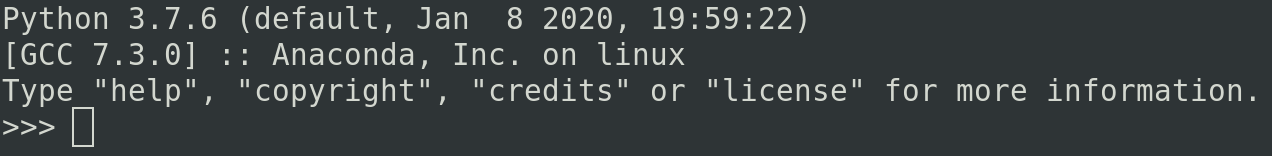
\includegraphics[width=10cm]{ressources/console.png}
\captionof{figure}{Console Python}
\label{console}
\end{figure}
\begin{activite}
\begin{enumerate}
\item Dans le dossier \emph{Maths} ou \emph{NSI} du bureau, ouvrir une console Python: \emph{Python 3.6.8}
\item Entrer les instructions ci -après (valider après chaque ligne):
\begin{lstlisting}
a = 12
b = 17
c = a + b
c
\end{lstlisting}
\item Expliquer le rôle de chaque ligne.
\end{enumerate}
\textbf{À retenir:} Le signe \textbf{=} n'est pas à comprendre au sens mathématique. C'est un signe d'affectation. Ainsi l'instruction
\begin{lstlisting}
12 = a
\end{lstlisting}
est juste mathématiquement mais ne signifie rien en Python.
\begin{enumerate}[resume]
\item Que renvoie l'instruction ci-après?
\begin{lstlisting}
c > 30
\end{lstlisting}
\end{enumerate}
\end{activite}
% insister sur différence boite / valeur: faire un exemple avec c = c+1
En première approche, nous pouvons considérer une \emph{variable} comme une boîte qui contient une information Cette information peut être de plusieurs natures (nombre, texte, tableau...)
\subsection{Entrée/sortie}
L'instruction
\begin{lstlisting}
input()
\end{lstlisting}
demande une valeur à l'utilisateur. Cependant la valeur est inaccessible. Il faut donc la stocker dans une variable en mémoire:
\begin{lstlisting}
age = input()
\end{lstlisting}
L'instruction
\begin{lstlisting}
print("mon texte")
\end{lstlisting}
affiche \emph{mon texte} à l'écran. Il est possible d'afficher le contenu d'une variable:
\begin{lstlisting}
print(age)
\end{lstlisting}
Il ne faut alors pas mettre de guillemets.
\begin{activite}
Écrire un programme qui demande l'âge de l'utilisateur, calcule l'année de naissance et affiche cette année.\\
\textbf{Aide:} Il sera nécessaire d'insérer l'appel \textbf{input()} dans une fonction \textbf{int()}. Nous reviendrons sur cet aspect.
\begin{lstlisting}
a = int(input())
\end{lstlisting}
\end{activite}
\begin{commentprof}
La valeur récupérée par \emph{input} est une chaîne de caractère.
\end{commentprof}
\subsection{Utilisation d'un EDI}
Il peut rapidement être fastidieux d'écrire un programme dans la console Python. Un \emph{Environnement de Développement Intégré} permettra d'écrire plusieurs lignes de code puis se chargera d'envoyer toutes ces lignes à l'interpréteur. De plus, il sera possible d'enregistrer le programme dans un fichier.
\begin{activite}
\begin{enumerate}
\item Dans l'espace personnel de l'ordinateur, créer un dossier \emph{NSI} et un sous-dossier \emph{langage}.
\item Ouvrir un EDI au choix: Spyder, Pyzo, EduPython. \emph{NB:} Les démonstrations au tableau seront réalisées avec Spyder.
\item Écrire le programme de l'activité 2 dans la partie gauche de l'EDI.
\item Enregistrer le programme dans le dossier \emph{NSI/langage} sous le nom \emph{naissance.py}
\item Exécuter le programme en cliquant sur la flèche verte (figure \ref{execution}) ou en appuyant sur la touche \emph{F5}. Le code est exécuté dans la console en bas à droite.
\end{enumerate}
\end{activite}
\begin{figure}[!h]
\centering

\includegraphics[width=1cm]{ressources/execution.png}
\captionof{figure}{Exécuter un programme}
\label{execution}
\end{figure}
\subsection{Structure conditionnelle}
En langage machine, il fallait comparer deux registres puis effectuer une action en fonction du résultat de la comparaison. Le comportement est similaire dans un langage de plus haut-niveau.
L'instruction
\begin{lstlisting}
a == b
\end{lstlisting}
renvoie \emph{True} si les variables \emph{a} et \emph{b} sont égales, \emph{False} sinon. Il faut noter l'emploi du \emph{double égal} pour ne pas confondre avec le signe d'affectation.\\
L'instruction
\begin{lstlisting}
if a == b:
    print(a)
\end{lstlisting}
compare \emph{a} et \emph{b} et affiche \emph{a} \textbf{si a == b}.
% insister sur l'évaluation qui est un booléen = donner l'ordre de l'interprétation par Python
\begin{activite}
\begin{enumerate}
\item Tester les codes ci-après:
\begin{lstlisting}
a = 5
b = 3
if a == b:
    print("a vaut ",a)
    print("b vaut ",b)
\end{lstlisting}
\begin{lstlisting}
a = 5
b = 3
if a == b:
    print("a vaut ",a)
print("b vaut ",b)
\end{lstlisting}
\item Noter les différences d'exécution.\\
\textbf{À retenir:} L'indentation a un rôle fondamental en Python. Par convention, on indente avec \emph{quatre espaces}. Il est possible d'utiliser la \emph{tabulation}, l'EDI se chargeant de la convertir en espaces.

\item Tester le code ci-après pour plusieurs valeurs de \emph{a} et \emph{b}. Bien observer l'indentation.
\begin{lstlisting}
a = 5
b = 3
if a == b:
    print("a et b sont égaux.")
else:
    print("a et b sont différents.")
\end{lstlisting}
\item Il est possible de tester plusieurs conditions. Trouver des valeurs de \emph{a} et \emph{b} pour lesquelles le message \guill{a est vraiment très grand.} est affiché.
\begin{lstlisting}
a = 5
b = 3
if a == b:
    print("a et b sont égaux.")
elif a > 10*b:
    print("a est vraiment très grand.")
else:
    print("a et b sont différents.")
\end{lstlisting}
\item Enregistrer le programme sous le nom \emph{condition.py}
\end{enumerate}
\end{activite}
\begin{commentprof}
attention aux mélanges espaces / tabulation dans des codes copiés depuis le net.
\end{commentprof}
\subsection{Répéter une instruction}
En langage machine, pour répéter des instructions il fallait créer un compteur, comparer ce compteur à la valeur limite et renvoyer le programme à une ligne précise.
\subsubsection{Boucle non bornée}
Une boucle \emph{non bornée} répète une instruction \emph{tant que} la condition est vérifiée.
\begin{activite}
\begin{enumerate}
\item Tester le programme ci-après:
\begin{lstlisting}
compteur = 10
while compteur > 0:
    print("Boum dans {} secondes.".format(compteur))
    compteur = compteur - 1
print("Boum")
\end{lstlisting}
\textbf{Tips:} Il est possible d'insérer des valeurs de variables dans du texte. Remarquer la structure de la ligne 3.
\item En anglais, que signifie \emph{while}?
\item À quelle ligne compare-t-on le compteur avec la valeur limite?
\item Quel est le rôle de la ligne 4? Que se passera-t-il si cette ligne est retirée?
\item Enregistrer le programme sous le nom \emph{boucle-non-bornee.py}
\end{enumerate}
\end{activite}
\begin{commentprof}
pour > 3.6: print(f"Boum dans {compteur} secondes.")
\end{commentprof}
\subsubsection{Boucle bornée}
Il existe une autre manière de répéter des instructions avec un mécanisme qui varie le compteur automatiquement.
\begin{activite}
\begin{enumerate}
\item Tester le programme ci-après:
\begin{lstlisting}
for compteur in range(10):
   print("Le compteur vaut {}".format(compteur))
\end{lstlisting}
\item Lire la documentation de la fonction \emph{range}:
\begin{center}
\url{https://docs.python.org/fr/3/tutorial/controlflow.html#the-range-function}
\end{center}
\item Adapter le code précédent pour afficher:
\begin{itemize}
\item Le compteur vaut 6.
\item Le compteur vaut 7.
\item Le compteur vaut 8.
\item Le compteur vaut 9.
\end{itemize}
\item Adapter le code précédent pour afficher:
\begin{itemize}
\item Le compteur vaut 0.
\item Le compteur vaut 3.
\item Le compteur vaut 6.
\item Le compteur vaut 9.
\end{itemize}
\item Enregistrer le programme sous le nom \emph{boucle-bornee.py}
\end{enumerate}
\end{activite}
\end{Form}
\end{document}